\documentclass{article}
\usepackage{graphicx}
\usepackage[margin=1.5cm]{geometry}
\usepackage{amsmath}

\begin{document}
\small
\title{Warm Up: Work and Energy}
\author{Prof. Jordan C. Hanson}

\maketitle

\section{Memory Bank}

\begin{itemize}
\item $KE = \frac{1}{2}m v^2$ ... Definition of Kinetic Energy
\item $W = KE_f - KE_i$ ... Work-energy theorem.
\item $U = mgy$ ... Gravitational potential energy.
\item $KE_i + PE_i = KE_f + PE_f$ ... One form of energy conservation.  Consider that potential energy is just stored energy created by performing work, so this statement is not that different from the official work-energy theorem.
\end{itemize}

\begin{figure}
\centering
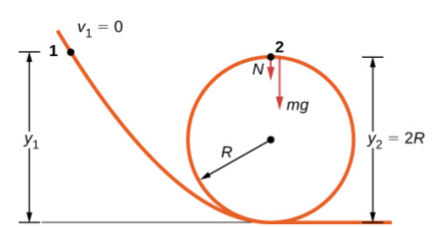
\includegraphics[width=0.45\textwidth]{figures/loop.png}
\caption{\label{fig:1} The classic loop-the-loop problem.}
\end{figure}

\section{Work and Energy}

\begin{enumerate}
\item In Fig. \ref{fig:1} below, a system begins with height $y_1$.  The zero-point of gravitational potential energy is located at the ground.  The system travels through the loop when released.  If $y_1$ is the minimum necessary height, we know that $N = 0$ at point 2.
\begin{itemize}
\item Start by writing down the \textit{gravitational potential energy} at points 1 and 2. \\ \vspace{1cm}
\item Assume that the system begins from rest.  What is $KE_i$? \\ \vspace{1cm}
\item Assume the system is moving at velocity $v$ at point 2, and has a mass $m$.  What is the kinetic energy? \\ \vspace{1cm}
\item At point 2, assume that the centripetal force is provided by the weight force, since $N = 0$.  Solve for $m v^2$. \\ \vspace{1cm}
\item Substitute everything into the energy conservation formula and solve for $y_1$.  If $y_1 = 80$ m, how fast will the system be moving at ground level?
\end{itemize}
\end{enumerate}

\end{document}
